\mubiaoline

\mubiaomu{1}{理解空间向量的相关概念（模、零向量、单位向量、相等向量、共线与共面），会用有向线段表示空间向量；}

\mubiaomu{2}{掌握空间向量线性运算（加减、数乘）的法则与运算律，理解共线、共面的充要条件；}

\mubiaomu{3}{掌握空间向量数量积的概念、性质与运算律，会求两向量的夹角与投影向量，并能用数量积求距离．}

\huaxing{课前预习}{预习自查\quad 温故知新}

\zsd{一}{空间向量的概念}

\tiaomu{1}{定义：在空间，我们把具有\kongbai{}和\kongbai{}的量叫做空间向量．}

\zhuzhu{与必修2平面向量初步的定义类比记忆（只多``空间''二字）；零向量方向任意、模为0，是概念题易错点。}

\tiaomu{2}{（1）字母表示法：用字母 \(\overrightarrow{a},\overrightarrow{b},\overrightarrow{c},\cdots\) 表示．（2）几何表示法：用有向线段表示，其\kongbai{}表示空间向量的模．即若向量 \(\overrightarrow{a}\) 的起点是 \(A\)、终点是 \(B\)，则向量 \(\overrightarrow{a}\) 也可记作 \(\overrightarrow{AB}\)，其模记为 \(\left| \overrightarrow{AB} \right|\)．}

\zhuzhu{字母表示与有向线段表示贯穿全章书写，解题前先统一记号；模的记号与绝对值区分，避免混淆。}

\tiaomu{3}{几类特殊向量（见下表）；规定：\kongbai{}向量与任意向量平行．即对任意向量 \(\overrightarrow{a}\)，都有 \(\overrightarrow{0}\parallel\overrightarrow{a}\)．}

\zhuzhu{概念辨析高频条目，判定按定义逐条核对；注意共线向量不要求在同一直线上（平行或重合均可），且零向量与任意向量平行（衔接条目5）。}

\noindent\hspace*{7mm}\begin{tabular}{|>{\raggedright\arraybackslash}p{16mm}|>{\raggedright\arraybackslash}p{34mm}|>{\raggedright\arraybackslash}p{22mm}|}
\hline
\multicolumn{1}{|>{\centering\arraybackslash}p{16mm}|}{\textbf{名称}} & \multicolumn{1}{|>{\centering\arraybackslash}p{34mm}|}{\textbf{定义}} & \multicolumn{1}{|>{\centering\arraybackslash}p{22mm}|}{\textbf{表示}} \\
\hline
零向量 & 长度为\kongbai{}的向量叫做零向量 & 记作\kongbai{} \\ \hline
单位向量 & 模等于\kongbai{}的向量 & 用 \(e\) 表示，\(|e|=1\) \\ \hline
相反向量 & 与 \(\overrightarrow{a}\) 长度相同而方向\kongbai{}的向量 & 记作 \(-\overrightarrow{a}\) \\ \hline
共线向量或平行向量 & 表示若干空间向量的有向线段所在的直线\kongbai{}或\kongbai{} & 记作 \(\overrightarrow{a}\parallel\overrightarrow{b}\) \\ \hline
相等向量 & 方向相同且\kongbai{}的向量 & 记作 \(\overrightarrow{a}=\overrightarrow{b}\) \\ \hline
\end{tabular}\par

\zsd{二}{空间向量的线性运算}

\tiaomu{4}{加法可按\kongbai{}法则或\kongbai{}法则作出；减法 \(\overrightarrow{a}-\overrightarrow{b}\) 为减向量终点指向被减向量终点；数乘 \(\lambda\overrightarrow{a}\)：当 \(\lambda>0\) 时与 \(\overrightarrow{a}\) 方向\kongbai{}，当 \(\lambda<0\) 时方向\kongbai{}，当 \(\lambda=0\) 时 \(\lambda\overrightarrow{a}=\overrightarrow{0}\)．}

\zhuzhu{全章运算的基础，加减、数乘的法则与运算律均与平面向量一致，类比迁移即可；线性组合的运用见条目9与10。}

\tiaomu{5}{共线的充要条件：对任意两个空间向量 \(\overrightarrow{a},\overrightarrow{b}\)（\(\overrightarrow{b}\neq\overrightarrow{0}\)），\(\overrightarrow{a}\parallel\overrightarrow{b}\) 的充要条件是存在\kongbai{} \(\lambda\)，使 \(\overrightarrow{a}=\lambda\overrightarrow{b}\)．}

\zhuzhu{证线线平行与求参数存在性的基础工具；易错点：与条目9共面充要条件混淆------共线用一个实数、共面用有序实数对。}

\noindent\hspace*{7mm}\begin{tabular}{|>{\raggedright\arraybackslash}p{16mm}|>{\raggedright\arraybackslash}p{34mm}|>{\raggedright\arraybackslash}p{22mm}|}
\hline
\multicolumn{1}{|>{\centering\arraybackslash}p{16mm}|}{\textbf{运算}} & \multicolumn{1}{|>{\centering\arraybackslash}p{34mm}|}{\textbf{法则要点}} & \multicolumn{1}{|>{\centering\arraybackslash}p{22mm}|}{\textbf{运算律举例}} \\
\hline
加法 & 三角形法则／平行四边形法则（与平面向量一致） & \(\overrightarrow{a}+\overrightarrow{b}=\overrightarrow{b}+\overrightarrow{a}\) \\ \hline
减法 & 减向量终点指向被减向量终点 & \((\overrightarrow{a}+\overrightarrow{b})+\overrightarrow{c}=\overrightarrow{a}+(\overrightarrow{b}+\overrightarrow{c})\) \\ \hline
数乘 & 实数 \(\lambda\) 与向量 \(\overrightarrow{a}\) 的乘积仍为向量 & \((\lambda+\mu)\overrightarrow{a}=\lambda\overrightarrow{a}+\mu\overrightarrow{a}\) \\ \hline
共线 & \(\overrightarrow{a}\parallel\overrightarrow{b}\)（\(\overrightarrow{b}\neq\overrightarrow{0}\)） & \(\overrightarrow{a}=\lambda\overrightarrow{b}\) \\ \hline
\end{tabular}\par

\zsd{三}{空间向量的夹角、数量积与共面}

\tiaomu{6}{夹角：已知两个非零向量 \(\overrightarrow{a},\overrightarrow{b}\)，在空间中任取一点 \(O\)，作 \(\overrightarrow{OA}=\overrightarrow{a},\overrightarrow{OB}=\overrightarrow{b}\)，则大小在\kongbai{}内的 \(\angle AOB\) 称为 \(\overrightarrow{a}\) 与 \(\overrightarrow{b}\) 的夹角，记作 \(\langle\overrightarrow{a},\overrightarrow{b}\rangle\)；当 \(\langle\overrightarrow{a},\overrightarrow{b}\rangle=\frac{\pi}{2}\) 时，称 \(\overrightarrow{a}\) 与 \(\overrightarrow{b}\)\kongbai{}，记作 \(\overrightarrow{a}\perp\overrightarrow{b}\)．}

\zhuzhu{夹角范围（0°到180°）是数量积正负讨论的前提；易混点：几何角（如异面直线所成角）与向量夹角可能互补，运算前先分清求的是哪个角。}

\tiaomu{7}{数量积：定义 \(\overrightarrow{a}\cdot\overrightarrow{b}=|\overrightarrow{a}||\overrightarrow{b}|\cos\langle\overrightarrow{a},\overrightarrow{b}\rangle\)；规定\kongbai{}与任意向量的数量积为 0．性质：\(\overrightarrow{a}\perp\overrightarrow{b}\Leftrightarrow\overrightarrow{a}\cdot\overrightarrow{b}=0\)；\(\overrightarrow{a}\cdot\overrightarrow{a}={{\overrightarrow{a}}^{2}}={\left| \overrightarrow{a} \right|}^{2}\)；\(\left| \overrightarrow{a}\cdot\overrightarrow{b} \right|\leq\left| \overrightarrow{a} \right|\left| \overrightarrow{b} \right|\)．}

\zhuzhu{【微提醒】零向量与任意向量的数量积为0．}

\zhuzhu{求空间角与距离的核心运算（支撑条目16、17、34）；注意数量积不满足结合律，零向量与任意向量的数量积为0。}

\bindp （1）在空间，向量\(\overrightarrow{a}\)向向量\(\overrightarrow{b}\)投影：

\bindp 如图①，先将它们平移到同一平面\(\alpha\)内，利用平面上向量的投影，得到与向量\(\overrightarrow{b}\)共线的向量\(\overrightarrow{c}\)，\(\overrightarrow{c} =\)\(\left| \overrightarrow{a} \right|\cos\left\langle \overrightarrow{a},\overrightarrow{b} \right\rangle \cdot \frac{\overrightarrow{b}}{\left| \overrightarrow{b} \right|}\)，称向量\(\overrightarrow{c}\)为向量\(\overrightarrow{a}\)在向量\(\overrightarrow{b}\)上的投影向量．

\bindp （2）向量\(\overrightarrow{a}\)在直线\emph{l}上的投影如图②．

\bindp \penalty10000\noindent\hspace*{7mm}\makebox[\dimexpr\linewidth-7mm\relax][c]{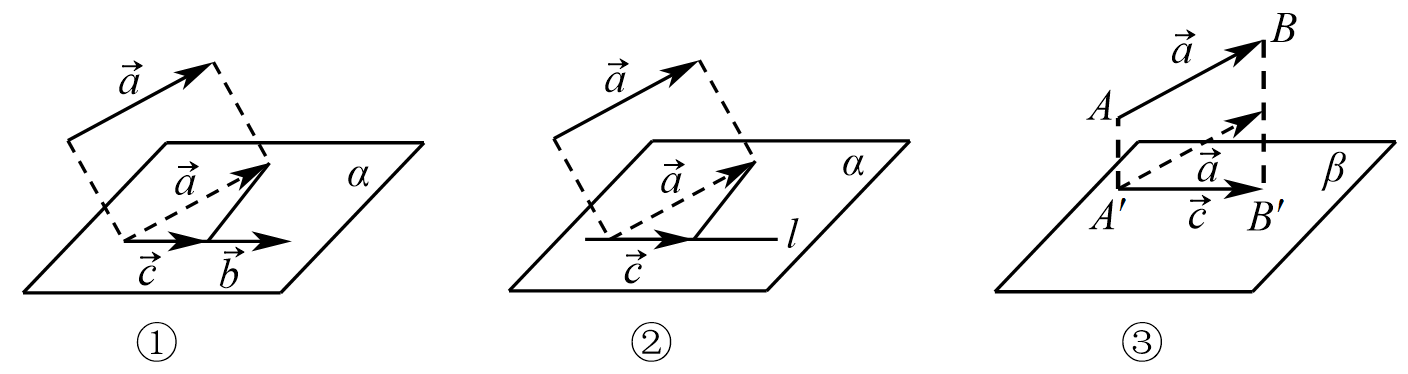
\includegraphics[width=45mm,alt={@@@5da5e1ea-9d33-4579-a56f-804b4a72c894}]{media/media/sub3_B_4.png}}\par\penalty10000

\bindp （3）向量\(\overrightarrow{a}\)向平面\(\beta\)投影：

\bindp 如图③，分别由向量\(\overrightarrow{a}\)的起点\emph{A}和终点\emph{B}作平面\(\beta\)的垂线，垂足分别为\(A'\)，\(B'\)，得到向量\(\overrightarrow{A'B'}\)，向量\(\overrightarrow{A'B'}\)称为向量\(\overrightarrow{a}\)在平面\(\beta\)上的投影向量．

\tiaomu{9}{共面的充要条件：向量 \(\overrightarrow{p}\) 与不共线向量 \(\overrightarrow{a},\overrightarrow{b}\) 共面的充要条件是存在\kongbai{} \((x,y)\)，使 \(\overrightarrow{p}=x\overrightarrow{a}+y\overrightarrow{b}\)．}

\zhuzhu{证四点共面、线共面的标准工具；易错点：定理前提是p与a、b不共线，此前提不可漏，且实数对存在唯一。}

\noindent\hspace*{7mm}\begin{tabular}{|>{\raggedright\arraybackslash}p{16mm}|>{\raggedright\arraybackslash}p{34mm}|>{\raggedright\arraybackslash}p{22mm}|}
\hline
\multicolumn{1}{|>{\centering\arraybackslash}p{16mm}|}{\textbf{概念}} & \multicolumn{1}{|>{\centering\arraybackslash}p{34mm}|}{\textbf{要点}} & \multicolumn{1}{|>{\centering\arraybackslash}p{22mm}|}{\textbf{记号／范围}} \\
\hline
夹角 & \(\angle AOB\)（\(\overrightarrow{OA}=\overrightarrow{a},\overrightarrow{OB}=\overrightarrow{b}\)） & \(0^\circ\leq\langle\overrightarrow{a},\overrightarrow{b}\rangle\leq180^\circ\) \\ \hline
数量积 & \(\overrightarrow{a}\) 的模与 \(\overrightarrow{b}\) 在 \(\overrightarrow{a}\) 上投影的数量之积 & \(\overrightarrow{a}\allowbreak\cdot\allowbreak\overrightarrow{b}\allowbreak=\allowbreak|\overrightarrow{a}|\allowbreak|\overrightarrow{b}|\allowbreak\cos\allowbreak\langle\overrightarrow{a},\overrightarrow{b}\rangle\) \\ \hline
投影向量 & 与 \(\overrightarrow{b}\) 同向（\(\cos\allowbreak\langle\overrightarrow{a},\overrightarrow{b}\rangle\allowbreak>0\) 时） & 模为 \(|\overrightarrow{a}|\allowbreak\cos\allowbreak\langle\overrightarrow{a},\overrightarrow{b}\rangle\) \\ \hline
共面 & 存在 \((x,y)\) 使 \(\overrightarrow{p}=x\overrightarrow{a}+y\overrightarrow{b}\)（\(\overrightarrow{a},\overrightarrow{b}\) 不共线） & \(\overrightarrow{p},\overrightarrow{a},\overrightarrow{b}\) 共面 \\ \hline
\end{tabular}\par

\zhenhead{判断正误（正确的打“√”，错误的打“×”）}

\zhenti{（一）}{相等向量一定是共线向量．}{\ansul{√}}

\zhenti{（二）}{若 \(\overrightarrow{a}\parallel\overrightarrow{b}\)，\(\overrightarrow{b}\parallel\overrightarrow{c}\)，则 \(\overrightarrow{a}\parallel\overrightarrow{c}\)．}{\ansul{×}}

\zhenti{（三）}{两个空间向量的模相等，则这两个向量相等．}{\ansul{×}}

\zhenti{（四）}{若 \(\overrightarrow{p}=x\overrightarrow{a}+y\overrightarrow{b}\)（\(\overrightarrow{a},\overrightarrow{b}\) 不共线），则 \(\overrightarrow{p},\overrightarrow{a},\overrightarrow{b}\) 共面．}{\ansul{√}}

\huaxing{课中探究}{例变探究\quad 素养提升}

\tjd{一｜空间向量的概念辨析}

\li{例1}{源 1.1.1.2-1·简单}{下列说法正确的是（~~~~）}

\bindopt A．若\(\left| \overrightarrow{a} \right| = \allowbreak\left| \overrightarrow{b} \right|\)，则\(\overrightarrow{a} = \overrightarrow{b}\)或\(\overrightarrow{a} = - \overrightarrow{b}\)；B．若\(\overrightarrow{a},\overrightarrow{b}\)为相反向量，则\(\overrightarrow{a} + \overrightarrow{b} = \overrightarrow{0}\) ；C．零向量是没有方向的向量；D．若\(\overrightarrow{a},\overrightarrow{b}\)是两个单位向量，则\(\overrightarrow{a} = \overrightarrow{b}\)

\bindp 【分析】根据零向量、单位向量、向量的模、相等向量、相反向量等概念逐一分析即可得出答案.

\bindp 【详解】解：若\(\left| \overrightarrow{a} \right| = \allowbreak\left| \overrightarrow{b} \right|\)，则它们的方向相同时是相等向量，方向相反时是相反向量，还有可能方向既不相同，也不相反，A错；

\bindp 若\(\overrightarrow{a},\overrightarrow{b}\)为相反向量，则它们的和为零向量，B对；

\bindp 零向量的方向是任意的，C错；

\bindp 两个单位向量只是模都为1，方向不一定相同，D错.故选：B.

\xiaojie{①识别：题干围绕模、方向、零向量、单位向量、相等向量与相反向量罗列说法要求辨误时，判归本题型。②操作：对照定义逐条核验，存疑条目用反例否定。③收束：排除错误项定答案，忌凭直觉误选。}

\tjd{二｜空间向量的线性运算}

\li{例1}{源 1.1.1.3-2·简单}{在直三棱柱\(ABC - A_{1}B_{1}C_{1}\)中，若\(\overrightarrow{CA} = \overrightarrow{a},\overrightarrow{CB} = \overrightarrow{b},\overrightarrow{CC_{1}} = \overrightarrow{c},\)，则\(\overrightarrow{A_{1}B}\)=\kongbai{}.(用\(\overrightarrow{a},\overrightarrow{b},\overrightarrow{c}\)表示)}

\bindp 【分析】连接\(CA_{1},\)根据直三棱柱的结构特征及空间向量减法的几何意义可得\(\overrightarrow{A_{1}B} = \overrightarrow{CB} - \overrightarrow{CA} - \overrightarrow{CC_{1}}\)，结合已知即可求表达式.

\bindp 【详解】连接\(CA_{1},\)则\(\overrightarrow{A_{1}B} = \overrightarrow{CB} - \overrightarrow{CA_{1}} = \overrightarrow{CB} - \overrightarrow{CA} - \overrightarrow{CC_{1}} =\)
\(\overrightarrow{b} - \overrightarrow{a} - \overrightarrow{c}\).

\bindp \penalty10000\noindent\hspace*{7mm}\makebox[\dimexpr\linewidth-7mm\relax][c]{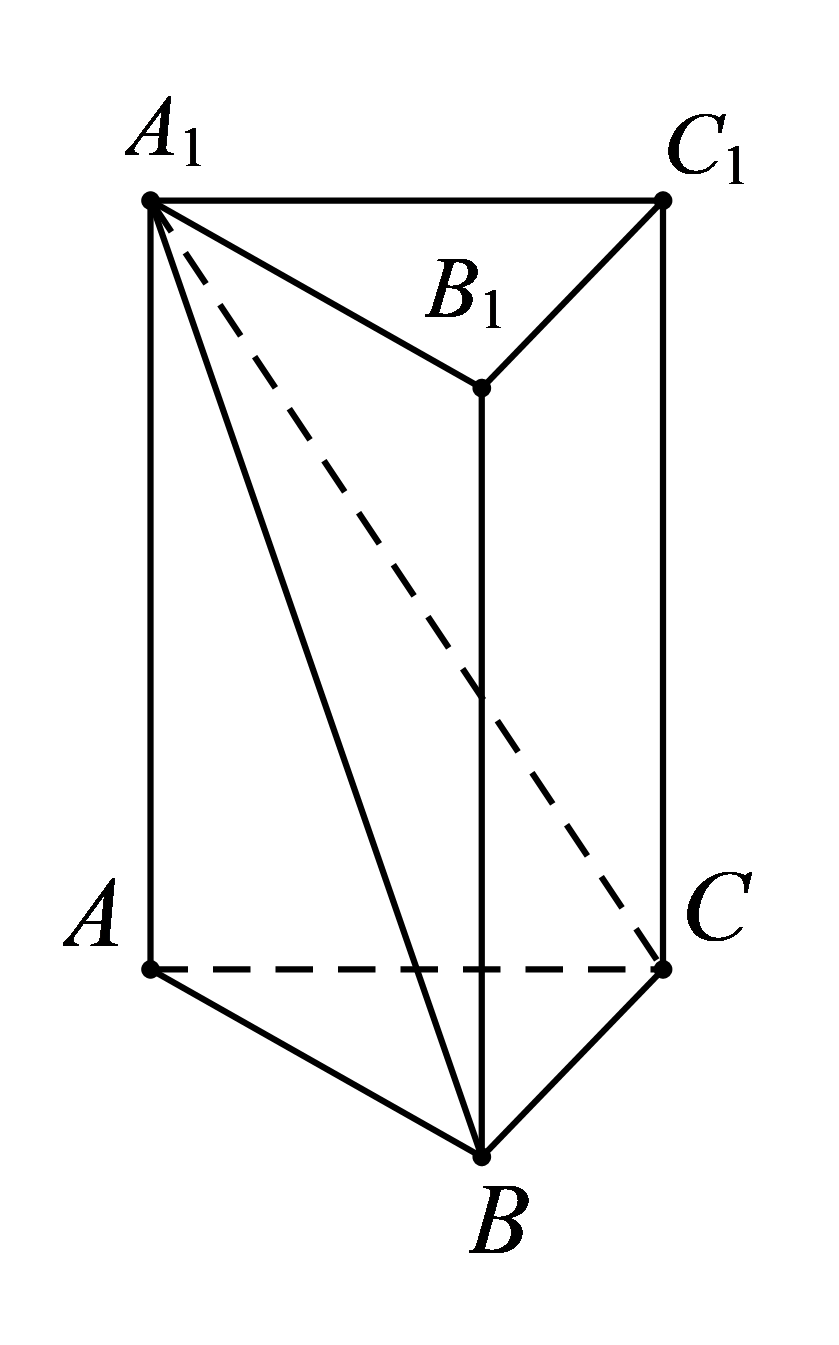
\includegraphics[width=30mm,alt={@@@4e3aa752498e415b9cc3d6d60f7bb3fe}]{media/media/image1.png}}\par\penalty10000

\bindp 故答案为：\(\overrightarrow{b} - \overrightarrow{a} - \overrightarrow{c}\)

\xiaojie{①识别：在几何体中给出若干已知向量、要求表示指定向量时，判归本题型。②操作：为目标向量选一条首尾相接的路径写出加减链，再把链中各段用相等或共线的已知向量替换，最后合并化简得表达式。③收束：复查每段方向与起讫点，防抄错向量。}

\tjd{三｜用基底表示向量}

\li{例1}{源 1.1.1.4-3·简单}{已知正方体\emph{ABCD}－\emph{A\textsubscript{1}B\textsubscript{1}C\textsubscript{1}D\textsubscript{1}}中，\(\overrightarrow{A_{1}E}\)＝\(\frac{1}{4}\) \(\overrightarrow{A_{1}C_{1}}\)，若\(\overrightarrow{AE} =\)\emph{x}\(\overrightarrow{AA_{1}}\)＋\emph{y}(\(\overrightarrow{AB}\)＋\(\overrightarrow{AD}\))，则\emph{x}＝\kongbai{}，\emph{y}＝\kongbai{}.}

\bindp \penalty10000\noindent\hspace*{7mm}\makebox[\dimexpr\linewidth-7mm\relax][c]{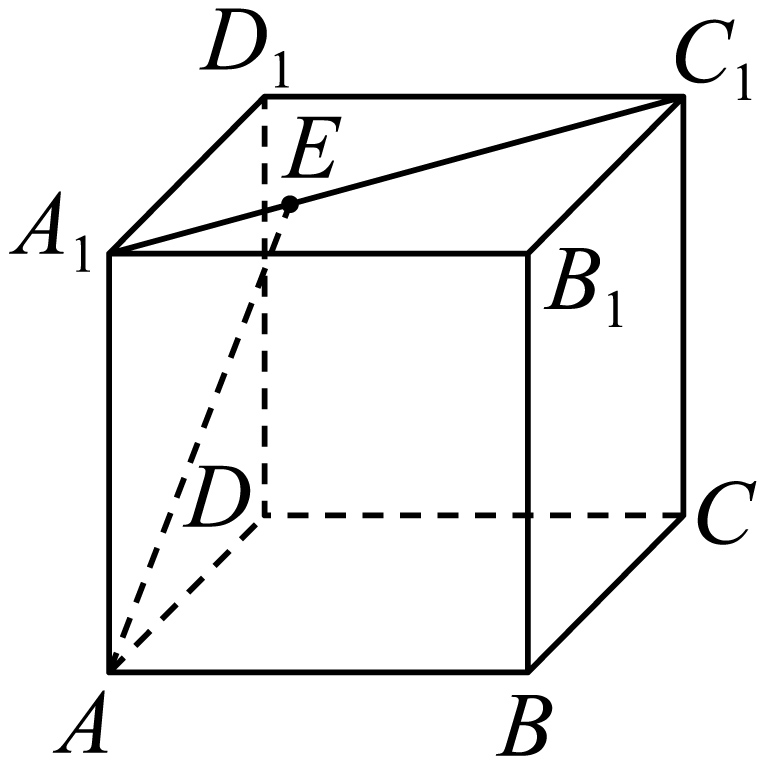
\includegraphics[width=30mm,alt={@@@b0b55c9f-4634-4bba-b096-bc6dd0cf7747}]{media/media/image2.png}}\par\penalty10000

\bindp 【分析】结合空间向量的线性运算列方程，由此求得\(x,y\)的值.

\bindp 【详解】\(\overrightarrow{AE} = \overrightarrow{AA_{1}} + \overrightarrow{A_{1}E} = \overrightarrow{AA_{1}} + \frac{1}{4}\overrightarrow{A_{1}C_{1}} = \overrightarrow{AA_{1}} + \frac{1}{4}\left( \overrightarrow{AB} + \overrightarrow{AD} \right)\)，所以\(x = 1,y = \frac{1}{4}\).故答案为：\(1\)；\(\frac{1}{4}\)

\xiaojie{①识别：指定三个不共面的向量作基底、要求把目标向量写成基底向量的线性组合并求系数时，判归本题型。②操作：先把目标向量沿几何路径分解为基底向量的和，再把各段按比例关系代入基底。③收束：比较等式两边系数求出待定值，防漏写中间段。}

\tjd{四｜共面向量的判定}

\xiaojie{①识别：题干给出 p=xa+yb 或 MP=xMA+yMB 一类线性表示与“共面”结论的互推说法判断时，判归本题型。②操作：核对充要条件的前提（两向量不共线或三点不共线）是否齐备，再对缺前提的说法举共线反例排除。③收束：最后汇总正确序号定选项。}

\tjd{五｜数量积的概念与运算律}

\li{例1}{源 1.1.1.6-5·简单}{设\(\overrightarrow{a}\)，\(\overrightarrow{b}\)为空间中的任意两个非零向量，下列各式中正确的有（~~~~）}

\bindopt A．\({\overrightarrow{a}}^{2} = \allowbreak\left| \overrightarrow{a} \right|^{2}\)；B．\(\frac{\overrightarrow{a} \cdot \overrightarrow{b}}{\overrightarrow{a} \cdot \overrightarrow{a}} = \frac{\overrightarrow{b}}{\overrightarrow{a}}\)；C．\(\left( \overrightarrow{a} \cdot \overrightarrow{b} \right)^{2} = {\overrightarrow{a}}^{2} \cdot {\overrightarrow{b}}^{2}\)；D．\(\left( \overrightarrow{a} - \overrightarrow{b} \right)^{2} = {\overrightarrow{a}}^{2} - 2\overrightarrow{a} \cdot \overrightarrow{b} + {\overrightarrow{b}}^{2}\)

\bindp 【分析】根据空间向量数量积的定义与运算律一一判断即可；

\bindp 【详解】解：对于A：\({\overrightarrow{a}}^{2} = \overrightarrow{a} \cdot \overrightarrow{a} = \allowbreak\left| \overrightarrow{a} \right| \cdot \allowbreak\left| \overrightarrow{a} \right|\cos 0 = \allowbreak\left| \overrightarrow{a} \right|^{2}\)，故A正确；

\bindp 对于B：因为向量不能做除法，即\(\frac{\overrightarrow{b}}{\overrightarrow{a}}\)无意义，故B错误；

\bindp 对于C：\(\left( \overrightarrow{a} \cdot \overrightarrow{b} \right)^{2} = \allowbreak\left( \left| \overrightarrow{a} \right| \cdot \allowbreak\left| \overrightarrow{b} \right|\cos\left\langle \overrightarrow{a},\overrightarrow{b} \right\rangle \right)^{2} = \allowbreak\left| \overrightarrow{a} \right|^{2} \cdot \allowbreak\left| \overrightarrow{b} \right|^{2}\cos^{2}\left\langle \overrightarrow{a},\overrightarrow{b} \right\rangle\)，故C错误；

\bindp 对于D：\(\left( \overrightarrow{a} - \overrightarrow{b} \right)^{2} = \allowbreak\left( \overrightarrow{a} - \overrightarrow{b} \right) \cdot \allowbreak\left( \overrightarrow{a} - \overrightarrow{b} \right) = {\overrightarrow{a}}^{2} - 2\overrightarrow{a} \cdot \overrightarrow{b} + {\overrightarrow{b}}^{2}\)，故D正确；故选：AD

\xiaojie{①识别：题干列出数量积相关的若干等式（平方、商式、乘积展开）要求判断正误时，判归本题型。②操作：按定义 a·b=|a||b|cosθ 逐式展开核验，展开后移项验算。③收束：警惕向量无除法、数量积无结合律等误用。}

\tjd{六｜数量积求夹角与投影（非坐标法）}

\xiaojie{①识别：题干在几何体中求两向量的夹角、模长或投影而不建坐标系时，判归本题型。②操作：先平移向量使起点共点或选不共面的三个向量作基底，再把相关向量用基底表示并算出数量积与模长。③收束：最后代入夹角公式并按向量夹角范围 [0,π] 取角。}

\tjd{七｜数量积条件求参（夹角与垂直）}

\li{例1}{源 1.1.1.8-7·中档}{已知向量\(\overrightarrow{a},\overrightarrow{b}\)，且\(\left| \overrightarrow{a} \right| = 2\)，\(\left| \overrightarrow{b} \right| = 1\)，\(\left\langle \overrightarrow{a},\overrightarrow{b} \right\rangle = 60^{\circ}\)，则使向量\(\overrightarrow{a} + \lambda\overrightarrow{b}\)与\(\lambda\overrightarrow{a} - 2\overrightarrow{b}\)的夹角为钝角的实数\(\lambda\)的取值范围是\kongbai{}．}

\bindp 【分析】根据\(\left( \overrightarrow{a} + \lambda\overrightarrow{b} \right) \cdot \allowbreak\left( \lambda\overrightarrow{a} - 2\overrightarrow{b} \right) < 0\)，得出方程求得\(- 1 - \sqrt{3} < \lambda < - 1 + \sqrt{3}\)，若向量\(\overrightarrow{a} + \lambda\overrightarrow{b}\)与\(\lambda\overrightarrow{a} - 2\overrightarrow{b}\)反向共线时，则存在实数\(k < 0\)使得\(\overrightarrow{a} + \lambda\overrightarrow{b} = k(\lambda\overrightarrow{a} - 2\overrightarrow{b})\)成立，得到方程组\(\left\{ \begin{array}{r}
k\lambda = 1 \\
\lambda = - 2k
\end{array} \right.\ \)无解，即可得到答案.

\bindp 【详解】由向量\(\overrightarrow{a},\overrightarrow{b}\)，且\(\left| \overrightarrow{a} \right| = 2\)，\(\left| \overrightarrow{b} \right| = 1\)，\(\left\langle \overrightarrow{a},\overrightarrow{b} \right\rangle = 60^{\circ}\)，可得\(\overrightarrow{a} \cdot \overrightarrow{b} = 2 \times 1 \times \cos 60^{\circ} = 1\)，

\bindp 因为向量\(\overrightarrow{a} + \lambda\overrightarrow{b}\)与\(\lambda\overrightarrow{a} - 2\overrightarrow{b}\)的夹角为钝角，可得\(\cos\left\langle \overrightarrow{a} + \lambda\overrightarrow{b},\lambda\overrightarrow{a} - 2\overrightarrow{b} \right\rangle < 0\)且\(\cos\left\langle \overrightarrow{a} + \lambda\overrightarrow{b},\lambda\overrightarrow{a} - 2\overrightarrow{b} \right\rangle \neq - 1\)，由\(\left( \overrightarrow{a} + \lambda\overrightarrow{b} \right) \cdot \allowbreak\left( \lambda\overrightarrow{a} - 2\overrightarrow{b} \right) < 0\)，即\(\lambda{\overrightarrow{a}}^{2}\text{+(}\lambda^{2} - 2)\overrightarrow{a} \cdot \overrightarrow{b} - 2\lambda{\overrightarrow{b}}^{2} < 0\)，所以\(\lambda^{2} + 2\lambda - 2 < 0\)，解得\(- 1 - \sqrt{3} < \lambda < - 1 + \sqrt{3}\)，

\bindp 若向量\(\overrightarrow{a} + \lambda\overrightarrow{b}\)与\(\lambda\overrightarrow{a} - 2\overrightarrow{b}\)反向共线时，存在实数\(k < 0\)，使得\(\overrightarrow{a} + \lambda\overrightarrow{b} = k(\lambda\overrightarrow{a} - 2\overrightarrow{b})\)成立，可得\(\left\{ \begin{array}{r}
k\lambda = 1 \\
\lambda = - 2k
\end{array} \right.\ \)，此时方程组无解，所以不存在实数\(k\)使得向量\(\overrightarrow{a} + \lambda\overrightarrow{b}\)与\(\lambda\overrightarrow{a} - 2\overrightarrow{b}\)反向共线，所以实数\(\lambda\)的取值范围是\(\left( - 1 - \sqrt{3}, - 1 + \sqrt{3} \right)\).

\li{变式1}{源 1.1.1.8-8·简单}{已知\(\left| \overrightarrow{a} \right| = 3\sqrt{2},\left| \overrightarrow{b} \right| = 4,\overrightarrow{m} = \overrightarrow{a} + \overrightarrow{b},\overrightarrow{n} = \overrightarrow{a} + \lambda\overrightarrow{b},\left\langle \overrightarrow{a},\overrightarrow{b} \right\rangle = 135{^\circ},\overrightarrow{m}\bot\overrightarrow{n}\) ，则λ＝\kongbai{}．}

\ansline{\(- \frac{3}{2}\)}

\xiaojie{①识别：题干给出两向量的模与夹角、并以夹角为锐角/钝角或两向量垂直为条件求参数时，判归本题型。②操作：第一步用数量积把条件翻译成不等式或方程（锐角 cos>0、钝角 cos<0、垂直 cos=0）。③收束：再求解并剔除使两向量共线的参数，最后写出参数值或取值范围。}

\tjd{八｜数量积求距离（展开法）}

\xiaojie{①识别：题干在含二面角的拼接图形中求两点距离时，判归本题型。②操作：第一步把待求线段对应的向量写成已知棱向量的首尾相接和链，再对模长平方作数量积展开，逐项代入模长与夹角（端点处两条垂线段的夹角由二面角决定，注意取 45° 还是 135°）。③收束：最后开方得距离。}

\tjd{九｜数量积求距离（折叠矩形）}

\xiaojie{①识别：题干为平面图形沿一条直线折起且折后两面垂直、求两点间距离时，判归本题型。②操作：第一步在折后图形中过两点对折痕作垂线定出垂足，再把目标向量写成两段垂线与折痕段的和链并平方展开。③收束：最后利用面面垂直带来的向量垂直逐项化简、开方得距离。}

\huaxing{课堂检测}{限时训练\quad 当堂达标}

\jiance{1．已知 \(|\overrightarrow{a}|=2\)，\(|\overrightarrow{b}|=3\)，\(\langle\overrightarrow{a},\overrightarrow{b}\rangle=60^\circ\)，则 \(\overrightarrow{a}\cdot\overrightarrow{b}=\)\kongbai{}．}{\ansul{3}}

\jiance{2．已知 \(\overrightarrow{a}=\overrightarrow{e_1}\allowbreak+\allowbreak2\overrightarrow{e_2}\)，\(\overrightarrow{b}=\allowbreak2\overrightarrow{e_1}\allowbreak-\allowbreak\overrightarrow{e_2}\allowbreak\)（\(\overrightarrow{e_1}\allowbreak,\allowbreak\overrightarrow{e_2}\) 不共线），判断 \(\overrightarrow{a}\) 与 \(\overrightarrow{b}\) 是否共线．}{\ansul{不共线}\allowbreak（设 \(\overrightarrow{a}=\lambda\overrightarrow{b}\) 得 \(\lambda=2\) 且 \(2\lambda=-1\)，矛盾）}
